\documentclass[conference]{IEEEtran}

\ifCLASSINFOpdf%

\else

\fi


\usepackage{graphicx}
\usepackage{textcomp}
\usepackage{mathtools}
\usepackage[backend=bibtex, style=ieee]{biblatex}
\usepackage{tabularx, caption}
\usepackage{hyperref}
\usepackage{tikz}

\def\layersep{2.5cm}
\tikzstyle{neuron}=[circle,fill=black!25,minimum size=17pt,inner sep=0pt]
\tikzstyle{input neuron}=[neuron, fill=green!50]
\tikzstyle{output neuron}=[neuron, fill=red!50]
\tikzstyle{hidden neuron}=[neuron, fill=blue!50]
\tikzstyle{annot}=[text width=4em, text centered]

\addbibresource{bibliography}

\begin{document}

\title{Data Mining --- Flavours of Physics}

\author{\IEEEauthorblockN{Selene Baez Santamaria (2572529) \\
		Andrea Jemmett (2573223) \\
		Dimitris Alivanistos (2578740)}

\IEEEauthorblockA{
Vrije Universiteit Amsterdam \\
Amsterdam, Netherlands}}

\maketitle


\begin{abstract}
%TODO
\end{abstract}


\IEEEpeerreviewmaketitle%


\section{Introduction}
\label{sec:intro}
% different techniques can be applied in one problem and the best on os not often obvious.
\texttt{Kaggle} \footnote{\url{https://www.kaggle.com/}} is a crowdsourcing platform where data mining and machine learning techniques are applied on open ended problems. It is the largest and most diverse data community in the world. In early 2016, the European Organization for Nuclear Research (CERN) launched a competition regarding the detection of an undiscovered phenomenon, called the charged lepton flavour violation \cite{hirsch2011charged}.

The Standard Model of particle physics considers symmetry to be a crucial property. However in many proposed extensions of that model this symmetry does not exist, implying that decays that do not conserve lepton flavour are possible. Observation of this decay would be a clear indication of the violation of lepton flavour and a sign of long-sought new physics.

\subsection{Objectives}
The domain of particle physics is complex and has been slowly developing for the past decades. Incorporating this knowledge into data mining techniques can be time consuming, specially if the data scientists has no prior experience in the field.

%TODO explain transfer learning is one of the chosen techniques taht can easily be applied without domain knowledge

Hence, the two main objectives of this paper are:

\begin{itemize}
	\item To implement a classification tool, without any particle physics domain knowledge, that has comparable performance to classifiers submitted to the competition.
	\item Experiment with ensemble models and transfer learning.
\end{itemize}

\subsection{Research question}
\label{sec:researchQuestions}
The research question to be explored is \textit{How does an uneducated ensemble model perform in the aforementioned Kaggle competition? How does it accuracy compare to other more domain knowledgeable classifiers?}

\subsection{Hypothesis}
\label{sec:hypothesis}
We believe that data mining is powerful enough to achieve comparable performance even without domain knowledge. Yet, we recognize that achieving such accuracy requires proper tuning and a careful design of structures.

Our hypothesis is that by investing enough time in experimenting and fine tuning our model, a competitive score can be achieved. We measure the competitiveness by Kaggle's ranking system, and expect to rank among the top five competitors.

\subsection{Contribution}
Although perfect score has already been achieved in this competition, the use of domain knowledge was crucial for it. Thus the main contribution of this paper is to prove that advance data mining techniques can alleviate our score to the one that the winners accomplished.

Furthermore, if our hypothesis proves to be correct, this work could be a stepping stone for applying data mining techniques in complex domains where knowledge is incomplete or uncertain. It could show the potential of data mining, by discovering patterns and insights, to boost scientific advances.

\subsection{Organization}
This project follows the Cross Industry Standard Process for Data Mining (CRISP-DT) Framework. As such, this paper's sections correspond to the six phases of the process model.

Section ~\ref{sec:intro} has introduced some Business Understanding related to High Energy Physics, specifically the need for proving the violation of charged lepton flavour. Furthermore, Section~\ref{sec:related_work} explores different existing data mining approaches of Kaggle top competitors. We continue to gain some Data Understanding by describing the dataset and the competition tools and regulations in Section~\ref{sec:dataset}. The Data Preparation and Modeling steps are outlined in Section~\ref{sec:system_design}, where the data is cleaned and the model implementation is described. To Evaluate the classifier, we set up several experiments as depicted in Sections~\ref{sec:experiment} and ~\ref{sec:results}. Finally, Section~\ref{sec:conclusion} summarizes our observations throughout the process.

\section{Related Work}
\label{sec:related_work}
In order to develop our solution for this competition we studied the approaches of other participants. Additionally, research was done to better understand the use of \textit{Ensemble Models} and \textit{Transfer Learning} in the context of solving a classification task.

\subsection{The Winner}
The winners of this competition were \textit{Vlad Mironov} and \textit{Alexander Guschin} of team Go Polar Bears. Their submission achieved 100\% accuracy by combining targeted solutions to the three main competition parts: improvement of the Area Under the Curve (AUC) score, and the given agreement and correlation tests.

Mironov and Guschin's model has two main characteristics to be noted. First, using scholar physics equations they recreated properties such as \textit{speed}, \textit{flight distance}, and \textit{mass}. This feature engineering step turned out to be crucial for the accuracy achieved. In fact, Vicens Gaitan, another participant ranked 14th in the competition, stated that other models, like Deep Networks, could build a mass-like property like the feature Mironov and Guschin engineered. Yet, Gaitan believes that the mass of a $\tau$ particle is hard to locate, even for this powerful methods.
%TODO add citation to his blog http://blog.kaggle.com/2015/10/27/passing-the-tests-strategies-used-in-cerns-flavour-of-physics/

Secondly, in order to significantly reduce the Mass correlation error, Mironov and Guschin used forests with \textit{Extreme Gradient Boosting}, a method used widely by data scientists to achieve state-of-the-art results on many machine learning challenges \cite{chen2016xgboost}. Parallelly, they used multilevel k-fold with bagging.

It is worth mentioning that the participants experimented with other configurations such as increasing the number of layers and neurons, however no significant changes in Area Under Curve were observed.

\subsection{Transfer learning solution}
The fifth ranked solution was submitted by Alexander Rakhlin and was based on transfer learning. This method assumes training and test data differ in some ways, a property extremely important for this specific competition. Furthermore, this method does not make ay domain specific assumptions and rather trains a model on a specific dataset and then applies this learned patterns? to a different dataset, regardless of their domain.
This is a fundamental difference from the winners' solution, since the model is not tailored to the Physics domain and their features are not manually engineered.

Ensemble of different neural networks. The three metrics AUC and the agreement and correlation metrics are taken into account into a loss function. This way, all of them are satisfied as result of statistical inference and not by coincidence.



\section{The Dataset}
\label{sec:dataset}
The competition provides a Starter Kit \footnote{\url{https://www.kaggle.com/c/flavours-of-physics/data}}, training and test sets, a specific
submission format and a couple check files to evaluate the submitted data. This competition was closed only eight months ago, and it is still relevant in the field.
%%%%%%
Given data from the Large Hadron Collider (LHC) a classification task needed to be performed in order to determine the presence for the variable \textit{signal}.  The data have been collected directly at the
LHC during experiments with high energy particles collisions. The dataset
consists of a collection of collision events and their properties. The objective
of the Kaggle competition was to predict whether a $\tau \rightarrow 3\mu$ decay
(the one that identifies a lepton flavour) was present in the collision. From
scientists this phenomenon is supposed \emph{not} to happen, so the goal of the
competition was to discover $\tau \rightarrow 3\mu$ happening more frequently
than scientists currently expect.

\subsection{Training Data}
For training there is a labeled dataset ready to be used to train a classifier.
The label, marked as \texttt{signal} with range in ${0,1}$ where 1 identifies
signal events while 0 represents background events. Signal events have been
simulated while background events come from real data collected by the LHCb
detectors, observing collision of accelerated particles with a specific mass
range in which $\tau \rightarrow 3\mu$ can't happen.

The training dataset is given is CSV format and contains 49 features plus target
label. For a detailed description of the features see
Appendix~\ref{sec:features}

\subsection{Testing}
For this Kaggle competition the submission procedure is different from the usual
ones. The dataset comes with, besides a test set, an \textit{agreement} and a
\textit{correlation} set. Any submission has to pass the agreement and
correlation checks before being scored on the test set.

\subsubsection{Agreement Test}
\label{sec:agreement}
The agreement dataset contains real and simulated events for a much more known,
observed and understood decay: $Ds \rightarrow \varphi\pi$. The motivation for
this check is that since the training set contains simulated data (for a
phenomenon not well understood), it is possible for the classifier to reach high
performances by picking up features that are not well modeled by the simulation.
The check then requires the classifier not to expose a large discrepancy when
applied to real-world and simulated data.

For this score, we are provided with a dataset on the control channel $Ds
\rightarrow \varphi\pi$ which has the same features as the training set. This
type of decay is not present in the training data. The
\textit{Kolmogorov-Smirnov} test is used to evaluate the differences between
real and simulated data between the classifier distribution on each sample.
The Kolmogorov-Smirnov metric has to be smaller than 0.09 to pass the agreement
check.

\subsubsection{Correlation Test}
\label{sec:correlation}
This test checks whether the classifier is uncorrelated with the $\tau$ mass.
Because mass is a measured quantity, scientists don't trust it when building a
model. Correlation with mass in an artificial signal-like peak or lead to
incorrect estimations of background signals.

The \texttt{mass} column is not included in the test dataset. However, this hidden
mass information is used to perform a \textit{Cramer-von Mises} test,
iteratively comparing two distributions of a.\ predicted values from submission
for entire dataset and b.\ predicted values within a certain mass region in
rolling window fashion along the whole mass range. Getting similar distributions
for all mass sub-regions means that the classifier is not correlated with the
mass. The submission must give a Cramer-von Mises value less than 0.002 to pass
the correlation test.

\subsubsection{Test Set}
\label{sec:test-set}
The test set has the same columns that the training set has except for
\texttt{mass}, \texttt{production}, \texttt{min\_ANNmuon} and \texttt{signal}.
The data contained in this dataset consists of:
\begin{enumerate}
	\item simulated signal events for $\tau \rightarrow 3\mu$;
	\item real background events for $\tau \rightarrow 3\mu$;
	\item simulated events for the $Ds \rightarrow \varphi\pi$;
	\item real background events for $Ds \rightarrow \varphi\pi$.
\end{enumerate}
Events related to the control channel are not used for scoring, but by the
agreement check (Section~\ref{sec:agreement}). One should treat all samples as
coming from the same collision channel during classification.

%TODO tal about preprocessing somewhere. Own section? subsection? just a sentence?

\section{System Design}
\label{sec:system_design}
The biggest challenge of this classification task is due to the evaluation
requirements. Since the training dataset contains both simulated and real-world
signals, the classifier is required to pass an agreement test. The purpose of
this test is to be sure that the distribution of predictions for real-world data
is similar to the one for simulated signals (recall that the test set comprehends
both $\tau \rightarrow 3\mu$ and $Ds \rightarrow \varphi\pi$ and competitors are
required to treat them equally during classification). The agreement test is
implemented by means of the Kolmogorov-Smirnov test, for which the required
metric has to be lower than 0.09. In a very similar way the classifier is
tested for correlation with the \texttt{mass} feature. This is because in physics the
mass of a particle is not believed to be a trustworthy feature when it comes to
building models. So a classifier has to pass a correlation test implemented
through a Cramer-von Mises test which has to return a score lower or equal to
0.002.

We build our model based on the Ensemble learning set of classifiers and apply
different variations and heuristics to the basic concepts, such as bagging and
stacking. The model consists of a composition of ensemble classifiers
implemented via Feed-forward Neural Networks, assembled together. The system
could be break down into two main stages: a first one where an ensemble of
Neural Networks is trained and used to produce predictions for all four datasets
(train, test, agreement and correlation); a second one where those predictions
are stacked with the original data to form an augmented dataset with as many new
features as networks in the first stage's ensemble (that is each data-point is
enriched with predictions from the ensemble).


\begin{figure}[h]
		\centering
		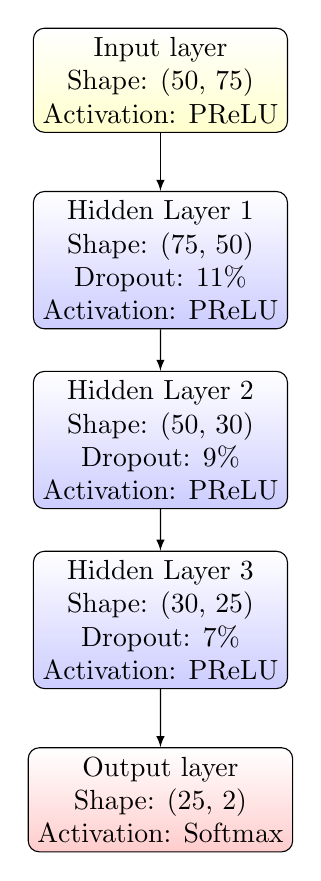
\begin{tikzpicture}[level distance=6.5em, edge from parent/.style={draw,-latex},
		every node/.style = {shape=rectangle, rounded corners, draw, align=center,
	top color=white, bottom color=blue!20}]]
			\node[bottom color=yellow!20] {Input layer \\ Shape: (50, 75) \\ Activation: PReLU}
			child { node {Hidden Layer 1 \\ Shape: (75, 50) \\ Dropout: 11\% \\ Activation: PReLU}
			child { node {Hidden Layer 2 \\ Shape: (50, 30) \\ Dropout: 9\% \\ Activation: PReLU}
			child { node {Hidden Layer 3 \\ Shape: (30, 25) \\ Dropout: 7\% \\ Activation: PReLU}
			child { node[bottom color=red!20] {Output layer \\ Shape: (25, 2) \\ Activation: Softmax}
			}}}};
		\end{tikzpicture}
		\caption{Neural Network configuration for the first stage (ensemble learning).}
		\label{fig:nn_ensemble_design}
\end{figure}


\subsection{Neural Networks design}
\label{sec:NN_design}
%TODO describe topologies and MOTIVATE THEM!
Each neural network consists of 5 fully connected layers. The first 4 layers
have a \textit{PReLU} activation function and the last one has a
\textit{softmax} function. Furthermore, layers 2, 3, and 4 perform Dropout in
order to avoid overfitting of the network. The input and output connections, as
well as summary of the above characteristics, is shown in the following table:

\begin{table}
	\centering
	\begin{tabular}[H]{ l c c c c }
		\textbf{Layer} & \textbf{\# inputs} & \textbf{\# outputs} &
			\textbf{Dropout rate} & \textbf{Activation function} \\ \hline
		\textit{Layer 1} & \# features & 75 & 0\% & PReLU \\
		\textit{Layer 2} & 75 & 50 & 11\% & PReLU \\
		\textit{Layer 3} & 50 & 30 & 9\% & PReLU \\
		\textit{Layer 4} & 30 & 25 & 7\% & PReLU \\
		\textit{Layer 5} & 25 & 2 & 0\% & softmax \\
	\end{tabular}
	\caption{Specification of the feed-forward Neural Network used in the first
		stage of training the classifier.}
	\label{tab:model1}
\end{table}

We use a \textit{Cross entropy} loss function.

\subsection{Model Ensemble}
The first stage of training the full classifier consists in training an ensemble
of feed-forward Neural Networks using the specifics from Table~\ref{tab:model1}.
Training is done only on the training set using the \textit{bootstrapping}
techniques, which consists in using a different sampled (with replacement)
version of the dataset to train each network in the ensemble. Bootstrapping is a
sampling technique used to obtain an approximation of independent and
identically distributed predictions and is the first step required to implement
\textit{bagging}, a technique to reduce the variance of the predictions.

After training is complete we generate predictions for all four datasets and
store them for the next stage. Predictions on the test set are also aggregated
using the mean to produce a \textit{majority vote} classification; this is a
simple implementation of bagging and unfortunately it is not sufficient to pass
the agreement and correlation tests.

\begin{table} % TODO change me!
	\centering
	\begin{tabular}{ l c c c c }
		\textbf{Layer} & \textbf{\# inputs} & \textbf{\# outputs} &
			\textbf{Dropout rate} & \textbf{Activation function} \\ \hline
		\textit{Layer 1} & \# features & 75 & 0\% & PReLU \\
		\textit{Layer 2} & 75 & 50 & 11\% & PReLU \\
		\textit{Layer 3} & 50 & 30 & 9\% & PReLU \\
		\textit{Layer 4} & 30 & 25 & 7\% & PReLU \\
		\textit{Layer 5} & 25 & 2 & 0\% & softmax \\
	\end{tabular}
	\caption{Specification of the feed-forward network used for transfer
		learning.}
	\label{tab:model2}
\end{table}

\subsection{Transfer Learning}
In the second stage of training we create a single Neural Network with the
specifications given in Table~\ref{tab:model2} and its weights are initialized
with an epoch of cross-entropy optimization on the training data. Then an
optimization algorithm (using scipy and Powell's method) is executed that tries
to minimize a loss function that incorporates AUC on the training set,
Kolmogorov-Smirnov on agreement set and Cramer-von Mises on the correlation set
in the following way:

\begin{align}
	\mathcal{L} &= -\text{AUC} + \text{KS} + \text{CvM}
	\label{eqn:loss}
\end{align}

The network is fed with the augmented data from the previous stage (original
data plus predictions from the previous stage).  After each optimization
iteration we check whether the KS and CvM metrics are less or equal to 0.09 and
0.002 respectively and that the AUC is greater than the previous stored one. If
all those three conditions are met, the network is stored for later use (e.g.
prediction).

Finally the generated ensemble of classifiers needs to be aggregated to form a
single prediction per data point. This is done again with the bagging technique,
by taking a majority vote (simple average in this case, because prediction
probabilities are required).

\section{Experimental set up}
\label{sec:experiment}

\subsection{Implementation}
\label{sec:implementation}


\subsection{Training}


\subsection{Testing/Evaluation}



\section{Results}
\label{sec:results}

\section{Conclusion}
\label{sec:conclusion}

\clearpage
\appendix

\section{Features for training}
\label{sec:features}
Follows a list of available features for training:
\begin{itemize}
	\item \texttt{FlightDistance}~-- distance between $\tau$ and PV (primary vertex, the
	original protons collision point);
	\item \texttt{FlightDistanceError}~-- error on FlightDistance;
	\item \texttt{mass}~-- reconstructed $\tau$ candidate invariant mass, which
	is \textit{absent in the test samples};
	\item \texttt{LifeTime}~-- life time of tau candidate;
	\item \texttt{IP}~-- Impact Parameter of tau candidate;
	\item \texttt{IPSig}~-- Significance of Impact Parameter;
	\item \texttt{VertexChi2}~-- $\chi^2$ of $\tau$ vertex;
	\item \texttt{dira}~-- cosine of the angle between the $\tau$ momentum and line
	between PV and tau vertex;
	\item \texttt{pt}~-- transverse momentum of $\tau$;
	\item \texttt{DOCAone}~-- Distance of Closest Approach between p0 and p1;
	\item \texttt{DOCAtwo}~-- Distance of Closest Approach between p1 and p2;
	\item \texttt{DOCAthree}~-- Distance of Closest Approach between p0 and p2;
	\item \texttt{IP\_p0p2}~-- Impact parameter of the p0 and p2 pair;
	\item \texttt{IP\_p1p2}~-- Impact parameter of the p1 and p2 pair;
	\item \texttt{isolationa}~-- track isolation variable;
	\item \texttt{isolationb}~-- track isolation variable;
	\item \texttt{isolationc}~-- track isolation variable;
	\item \texttt{isolationd}~-- track isolation variable;
	\item \texttt{isolatione}~-- track isolation variable;
	\item \texttt{isolationf}~-- track isolation variable;
	\item \texttt{iso}~-- track isolation variable;
	\item \texttt{CDF1}~-- cone isolation variable;
	\item \texttt{CDF2}~-- cone isolation variable;
	\item \texttt{CDF3}~-- cone isolation variable;
	\item \texttt{production}~-- source of $\tau$ (\textit{absent from test data});
	\item \texttt{ISO\_SumBDT}~-- track isolation variable;
	\item \texttt{p0\_IsoBDT}~-- track isolation variable;
	\item \texttt{p1\_IsoBDT}~-- track isolation variable;
	\item \texttt{p2\_IsoBDT}~-- track isolation variable;
	\item \texttt{p0\_track\_Chi2Dof}~-- quality of p0 muon track;
	\item \texttt{p1\_track\_Chi2Dof}~-- quality of p1 muon track;
	\item \texttt{p2\_track\_Chi2Dof}~-- quality of p2 muon track;
	\item \texttt{p0\_pt}~-- transverse momentum of p0 muon;
	\item \texttt{p0\_p}~-- momentum of p0 muon;
	\item \texttt{p0\_eta}~-- pseudorapidity of p0 muon;
	\item \texttt{p0\_IP}~-- Impact parameter of p0 muon;
	\item \texttt{p0\_IPSig}~-- Impact Parameter Significance of p0 muon;
	\item \texttt{p1\_pt}~-- transverse momentum of p1 muon;
	\item \texttt{p1\_p}~-- momentum of p1 muon;
	\item \texttt{p1\_eta}~-- pseudorapidity of p1 muon;
	\item \texttt{p1\_IP}~-- Impact parameter of p1 muon;
	\item \texttt{p1\_IPSig}~-- Impact Parameter Significance of p1 muon;
	\item \texttt{p2\_pt}~-- transverse momentum of p2 muon;
	\item \texttt{p2\_p}~-- momentum of p2 muon;
	\item \texttt{p2\_eta}~-- pseudorapidity of p2 muon;
	\item \texttt{p2\_IP}~-- Impact parameter of p2 muon;
	\item \texttt{p2\_IPSig}~-- Impact Parameter Significance of p2 muon;
	\item \texttt{SPDhits}~-- number of hits in the SPD detector;
	\item \texttt{min\_ANNmuon}~-- muon identification. LHCb collaboration trains
  	Artificial Neural Networks (ANN) from informations from RICH, ECAL,
  	HCAL, Muon system to distinguish muons from other particles. This
  	variable denotes the minimum of the three muons ANN. This feature
  	should not be used for training and is \textit{absent from the test
		sets};
	\item \texttt{signal}~-- is the target variable to predict.
\end{itemize}

\printbibliography

\end{document}
